\section{Results}
\label{sec:results}

\subsection{Experiment 1: Synthetic Data Has Lower Perplexity}
\label{sec:results_exp1}

\begin{table}[t]
    \centering
    \caption{Perplexity statistics for human and synthetic data as measured by the base \gptsmall model. Synthetic data has $3\times$ lower median perplexity, confirming that the model finds its own output far more predictable. The high synthetic mean is driven by outliers from EOS-padded sequences; the median is the informative comparison.}
    \begin{tabular}{@{}lccc@{}}
        \toprule
        \textbf{Data Source} & \textbf{Mean PPL} & \textbf{Median PPL} & \textbf{Std PPL} \\
        \midrule
        Human    & 45.0  & 43.2           & 15.8 \\
        Synthetic & 7{,}603.3 & \textbf{14.6} & 43{,}043.5 \\
        \bottomrule
    \end{tabular}
    \label{tab:perplexity}
\end{table}

\Tabref{tab:perplexity} summarizes the perplexity distributions. Synthetic data has a median perplexity of 14.6 compared to 43.2 for human data---a $3\times$ reduction. The Mann-Whitney $U$ test confirms this difference is highly significant ($U = 2{,}170{,}034$, $p < 10^{-282}$). \Figref{fig:perplexity} shows the full distributions: human data perplexity is concentrated in a relatively tight band around the median, while synthetic data is strongly left-skewed with a long right tail from degenerate sequences.

\begin{figure}[t]
    \centering
    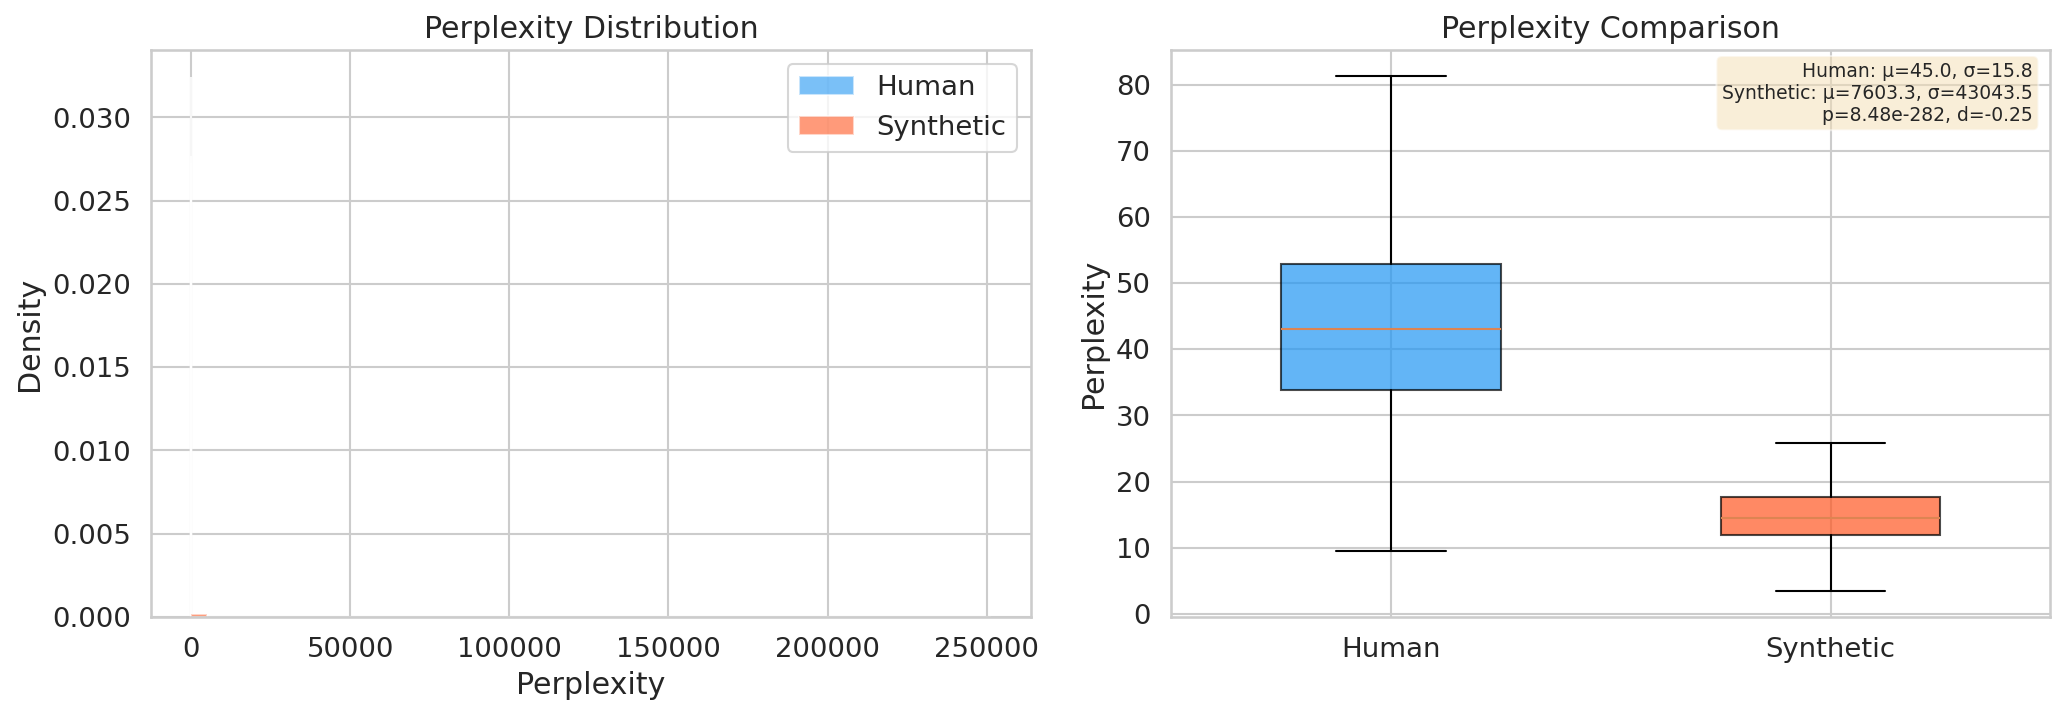
\includegraphics[width=0.95\linewidth]{figures/fig1_perplexity_distributions.png}
    \caption{Perplexity distributions for human and synthetic data. The synthetic distribution is strongly concentrated at low perplexity values, confirming that the model finds its own output highly predictable. The long right tail reflects degenerate sequences with EOS padding.}
    \label{fig:perplexity}
\end{figure}

This result establishes the premise of our hypothesis: the model's own output is far more predictable than human text, which should translate into smaller loss values and consequently smaller gradients.

\subsection{Experiment 2: Synthetic Data Produces Smaller Gradients}
\label{sec:results_exp2}

\begin{table}[t]
    \centering
    \caption{Gradient $L^2$ norm statistics over 200 fine-tuning steps. Human data produces 15\% larger gradients on average, with high statistical significance.}
    \begin{tabular}{@{}lccc@{}}
        \toprule
        \textbf{Data Source} & \textbf{Mean $\|\vg\|_2$} & \textbf{Std} & \textbf{Ratio} \\
        \midrule
        Human    & 3.856 & 0.638 & \multirow{2}{*}{\textbf{1.15$\times$}} \\
        Synthetic & 3.362 & 0.909 & \\
        \bottomrule
    \end{tabular}
    \label{tab:gradnorms}
\end{table}

\Tabref{tab:gradnorms} shows that human data produces gradient norms that are 15\% larger on average (3.856 vs.\ 3.362). The Mann-Whitney $U$ test yields $U = 36{,}261$ with $p = 3.14 \times 10^{-45}$, and Cohen's $d = 0.629$ indicates a medium effect size. \Figref{fig:gradnorms} shows the gradient norms across training steps: the human-data trajectory is consistently above the synthetic-data trajectory.

\begin{figure}[t]
    \centering
    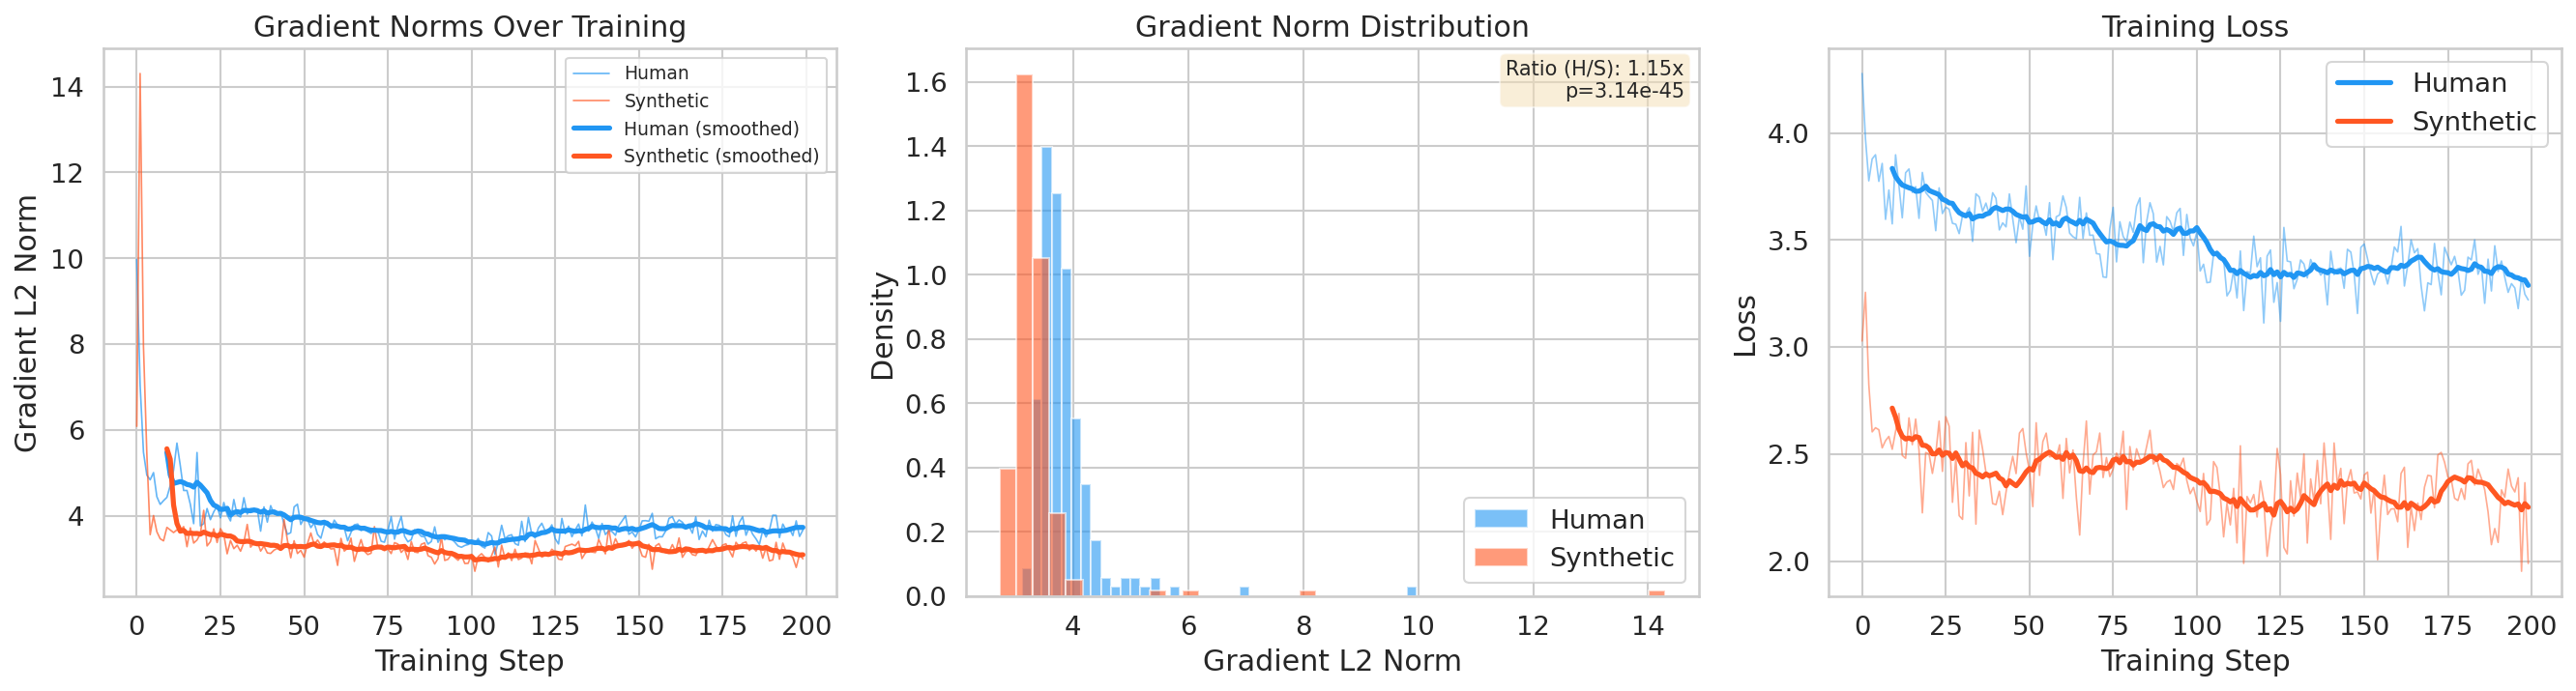
\includegraphics[width=0.95\linewidth]{figures/fig2_gradient_norms.png}
    \caption{Gradient $L^2$ norms over 200 fine-tuning steps for human and synthetic data. Human data consistently produces larger gradients. The effect is stable across training, not a transient phenomenon.}
    \label{fig:gradnorms}
\end{figure}

While statistically significant, the 15\% norm reduction alone does not fully explain the large efficiency gaps we observe in Experiment~4. This motivates the directional analysis in Experiment~3, which reveals a far more dramatic difference.

\subsection{Experiment 3: Gradient Directional Collapse}
\label{sec:results_exp3}

\begin{table}[t]
    \centering
    \caption{Gradient direction analysis across four attention weight matrices. \textbf{Rank-90\%}: number of PCA components to explain 90\% of gradient variance. \textbf{Cos Sim}: average pairwise cosine similarity among gradients within each condition. \textbf{Overlap}: cosine similarity between the top principal subspaces of human and synthetic gradients. Synthetic gradients occupy a dramatically lower-dimensional subspace in 3 of 4 layers. Best (most concentrated) rank values in \textbf{bold}.}
    \resizebox{\textwidth}{!}{%
    \begin{tabular}{@{}lcccccc@{}}
        \toprule
        & \multicolumn{2}{c}{\textbf{Rank-90\%}} & \multicolumn{2}{c}{\textbf{Cos Sim}} & \\
        \cmidrule(lr){2-3} \cmidrule(lr){4-5}
        \textbf{Layer} & Human & Synthetic & Human & Synthetic & \textbf{Overlap} \\
        \midrule
        \texttt{h.0.c\_attn}  & 51 & \textbf{2}  & 0.608 & 0.691 & 0.131 \\
        \texttt{h.5.c\_attn}  & 51 & 30 & 0.812 & 0.726 & 0.318 \\
        \texttt{h.11.c\_attn} & 51 & \textbf{1}  & 0.654 & 0.722 & 0.157 \\
        \texttt{h.11.c\_proj} & 51 & \textbf{1}  & 0.617 & 0.709 & 0.283 \\
        \bottomrule
    \end{tabular}
    }
    \label{tab:directions}
\end{table}

\Tabref{tab:directions} presents our central finding. In 3 of 4 layers, synthetic data gradients need only \textbf{1--2 PCA components} to explain 90\% of variance, compared to \textbf{51 components} (the maximum measured) for human data. This represents a striking directional collapse: synthetic gradients are essentially one-dimensional, while human gradients span a rich, high-dimensional subspace.

Three additional patterns emerge:

\para{Higher internal consistency.} Synthetic gradients have higher average pairwise cosine similarity (0.69--0.73) than human gradients (0.61--0.65), confirming that synthetic batches push the model in more consistent---and thus more redundant---directions.

\para{Low subspace overlap.} The overlap between human and synthetic gradient subspaces is very low (0.13--0.32), meaning the directions that synthetic data reinforces are largely \emph{different} from those that human data reinforces. This is not simply a case of synthetic gradients being a subset of human gradient directions; they occupy a qualitatively different region of parameter space.

\para{Layer-specific dynamics.} The middle layer (\texttt{h.5}) shows a qualitatively different pattern: synthetic gradients use 30 components (vs.\ 1--2 in other layers) and human gradients show unusually high internal similarity (0.812). This suggests middle layers process more structural or syntactic features where human and synthetic text are more similar, while early and late layers capture distributional differences that synthetic data homogenizes.

\begin{figure}[t]
    \centering
    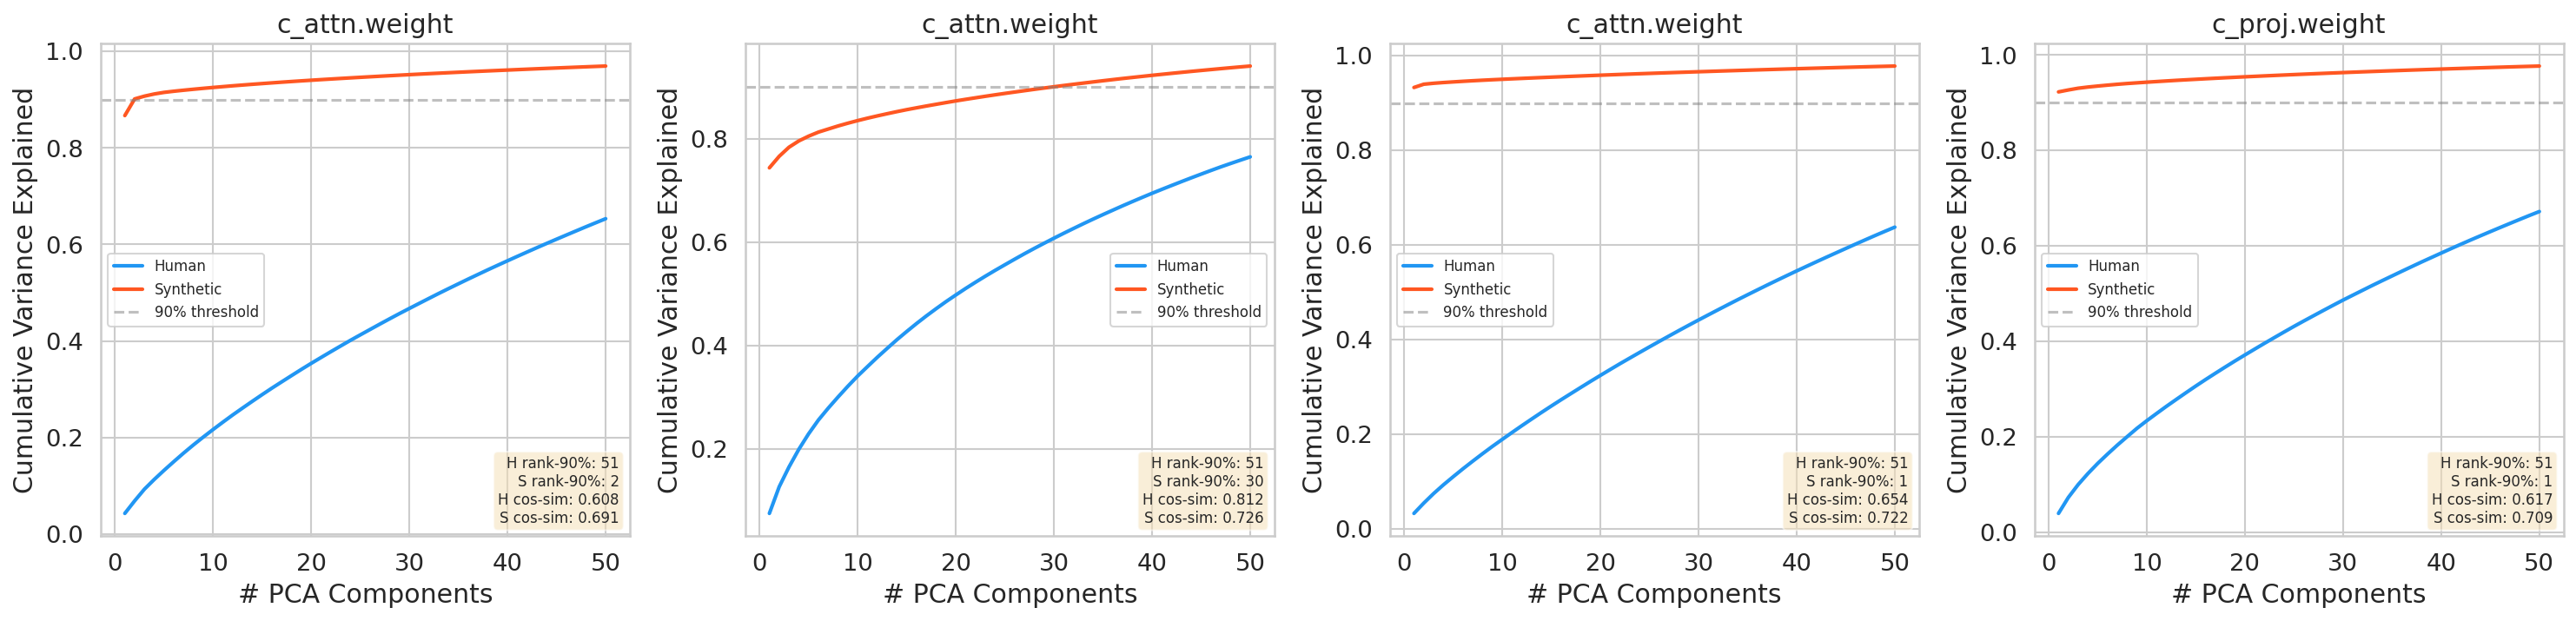
\includegraphics[width=0.95\linewidth]{figures/fig3_gradient_directions.png}
    \caption{PCA analysis of gradient directions for human and synthetic data across four attention layers. Synthetic gradients cluster tightly along a single direction, while human gradients span a broad subspace. The separation is most pronounced in early (\texttt{h.0}) and late (\texttt{h.11}) layers.}
    \label{fig:directions}
\end{figure}

\begin{figure}[t]
    \centering
    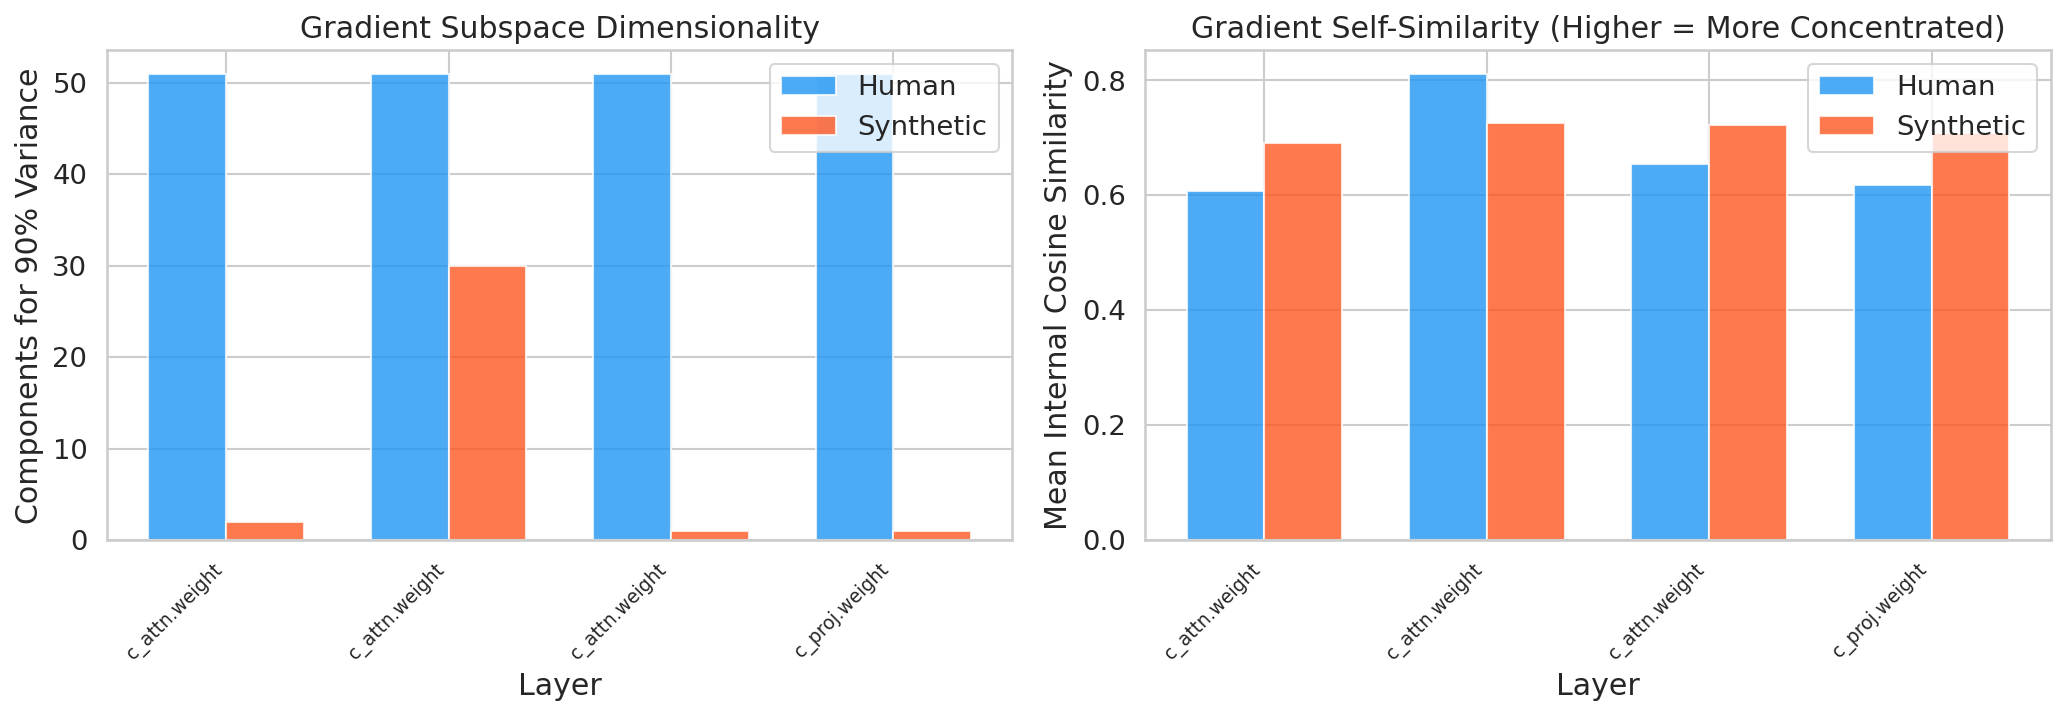
\includegraphics[width=0.95\linewidth]{figures/fig3b_direction_summary.png}
    \caption{Summary of gradient direction metrics across layers. \figleft Effective rank (components for 90\% variance) shows the dramatic dimensionality gap between human and synthetic gradients. \figright Subspace overlap is consistently low, indicating human and synthetic gradients drive learning in largely orthogonal directions.}
    \label{fig:direction_summary}
\end{figure}

\subsection{Experiment 4: Reduced Sample Efficiency}
\label{sec:results_exp4}

\begin{table}[t]
    \centering
    \caption{Validation perplexity on human \wikitext data after 200 fine-tuning steps at varying data scales. Synthetic data consistently achieves worse perplexity, with the gap widening at smaller data scales. Lower is better.}
    \begin{tabular}{@{}lccc@{}}
        \toprule
        \textbf{Data Fraction} & \textbf{Human Val PPL} & \textbf{Synthetic Val PPL} & \textbf{Ratio} \\
        \midrule
        10\% (158 seqs)   & \textbf{80.7}  & 142.8 & 1.77$\times$ \\
        25\% (395 seqs)   & \textbf{40.7}  & 64.1  & 1.58$\times$ \\
        50\% (790 seqs)   & \textbf{33.4}  & 48.6  & 1.46$\times$ \\
        100\% (1{,}581 seqs) & \textbf{30.8}  & 43.1  & 1.40$\times$ \\
        \bottomrule
    \end{tabular}
    \label{tab:efficiency}
\end{table}

\Tabref{tab:efficiency} shows that synthetic data achieves worse validation perplexity at every data scale. The efficiency gap is most pronounced at small data sizes ($1.77\times$ at 10\%) and narrows at larger scales ($1.40\times$ at 100\%). Even with 100\% of the synthetic data, the model achieves only the perplexity level that human data reaches at roughly 25--50\% scale. \Figref{fig:efficiency} shows the learning curves.

\begin{figure}[t]
    \centering
    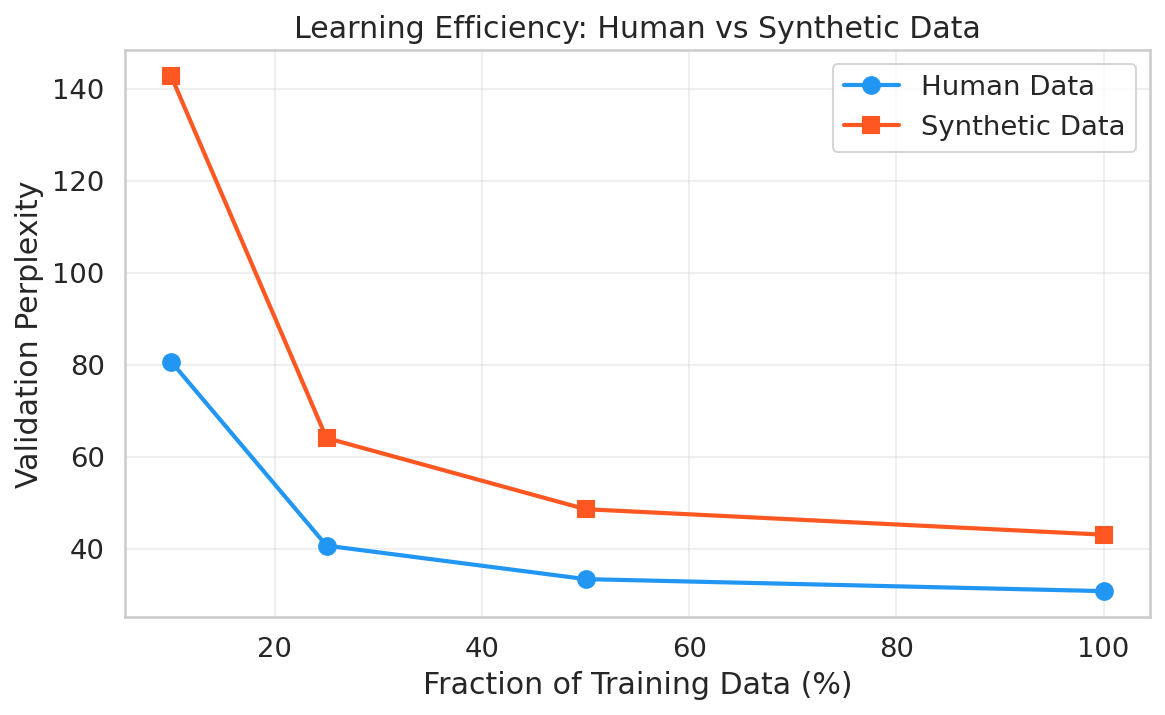
\includegraphics[width=0.95\linewidth]{figures/fig4_learning_efficiency.png}
    \caption{Validation perplexity versus data fraction for human and synthetic training data. The gap widens at smaller data scales, consistent with the gradient attenuation mechanism: when data is scarce, the weaker and narrower gradient signal from synthetic data is especially insufficient.}
    \label{fig:efficiency}
\end{figure}

The widening gap at small data scales is consistent with the gradient attenuation mechanism. When data is scarce, each batch matters more. If those batches produce gradients concentrated in just 1--2 directions (as Experiment~3 shows), the model updates only a tiny fraction of its parameters meaningfully, wasting the limited data budget.
